\documentclass[a4paper, twoside, english]{article}

\usepackage{amsmath}
\usepackage{amsfonts}
\usepackage{ihci}
\usepackage{graphicx}
\usepackage{subfig}

\graphicspath{{./../figures/}}

\title{Exercise 1 \\ 3D Computer Vision}  % Replace "Template Report" with Exercise 1, Exercise 2, etc
\author{Albert Garaev, Ksenia Novikova, Mukhammadsodik Khabibulloev }    % Replace with your names
\date{09.11.2021}                              % Replace with current date

\begin{document}

\maketitle

\section{Introduction}

This report presents the results of the theoretical and practical parts of Exercise 1.

\section{Theory}
\subsection{ Properties of Rotation Matrices}
\textit{(a) The task is showing the fact that the rows and columns of R are orthonomal\\ (orthogonal and of length 1).}\\
Let's begin with the rotation matrix around the x-axis.\\
Rotation by $\phi$ aroud $x$ axis:
\begin{equation}
	R_x = \left[
	\begin{array}{ccc}
		1 & 0 & 0 \\
		0 & cos \phi & -sin \phi \\
		0 & sin \phi & cos \phi
	\end{array}
	\right].
	\label{eq:kmatrixX}
\end{equation}
We can prove that the rows and columns of $R$ are orthogonal by proving the equations $R^{-1} = R^T$ and $det(R)=1.$
Let's calculate ${{R_x}^{-1}}={{(R_x^{*})^T}\over{det(R_x)}}$, we need to calculate $det(R_x)$ using minors M.

${det(R_x)=(using\ first\ row)=1*(cos \phi * cos \phi - (-sin \phi * sin \phi)) - 0 + 0 = \cos^2 \phi + \sin^2 \phi = 1}$\\
Find transposed matrix $R_x^T$:
\begin{equation*}
	{R_x^T} = \left[
	\begin{array}{ccc}
		1 & 0 & 0 \\
		0 & cos \phi & sin \phi \\
		0 & -sin \phi & cos \phi
	\end{array}
	\right]
	\label{eq:kmatrixXT}
\end{equation*}
Find minor matrix M:
\begin{equation*}
	M=\left[
	\begin{array}{ccc}
		1&0&0\\
		0&\cos\phi&\sin\phi\\
		0&-\sin\phi&\cos\phi
	\end{array}
	\right]
\end{equation*}
Find adjugate matrix $R_x^{*}$:
\begin{equation*}
R_x^{*}=	\left[
	\begin{array}{ccc}
		1&0&0\\
		0&\cos\phi&-\sin\phi\\
		0&\sin\phi&\cos\phi
	\end{array}
	\right]
\end{equation*}
Thus, we can find the value of ${R_x}^{-1}$
\begin{equation*}
{{R_x}^{-1}}={{(R_x^{*})^T}\over{det(R_x)}}= {{\left[ \begin{array}{ccc}
	1 & 0 & 0 \\
	0 & cos \phi & sin \phi \\
	0 & -sin \phi & cos \phi
\end{array} \right]}\over {1}} =  {\left[ \begin{array}{ccc}
1 & 0 & 0 \\
0 & cos \phi & sin \phi \\
0 & -sin \phi & cos \phi
\end{array} \right]} = R^T
\end{equation*} Q.E.D.\\
Now we will prove that the length of any row or column is equal to 1.\\
 {Row 1 $r_1=(1,0,0)$. ${{|r_1|}={\sqrt{1^2+0^2+0^2}}=1}$}\\
 {Row 2 $r_2=(0, cos \phi , -sin \phi )$. ${|r_2|}={\sqrt{0^2+(\cos\phi)^2+(-\sin \phi)^2}}={\sqrt{ \cos^2 \phi + \sin^2 \phi}} = 1$}\\
 {Row 3 $r_3=(0, sin \phi , cos \phi )$. ${|r_3|}={\sqrt{0^2+(\sin\phi)^2+(\cos \phi)^2}}={\sqrt{ \sin^2 \phi + \cos^2 \phi}} = 1$}\\
 {Column 1 $c_1=(1,0,0)$. ${|c_1|}={\sqrt{1^2+0^2+0^2}}=1$}\\
 {Column 2 $c_2=(0, cos \phi , sin \phi )$. ${|c_2|}={\sqrt{0^2+(\cos\phi)^2+(\sin \phi)^2}}={\sqrt{ \cos^2 \phi + \sin^2 \phi}} = 1$}\\
 {Column 3 $c_3=(0,-sin \phi , cos \phi )$. ${|c_3|}={\sqrt{0^2+(-\sin\phi)^2+(\cos \phi)^2}}={\sqrt{ \sin^2 \phi + \cos^2 \phi}} = 1$}\\\\
Thus, since rows and columns of matrix $R_x$ are orthogonal and their length is equal to 1, we prove that they are orthonormal.

Now consider the rotation matrix around the y-axis.\\
Rotation by $\theta$ aroud $y$ axis:
\begin{equation}
	R_y = \left[
	\begin{array}{ccc}
		cos \theta & 0 & sin \theta \\
		0 & 1 & 0 \\
		-sin \theta & 0 & cos \theta
	\end{array}
	\right].
	\label{eq:kmatrixY}
\end{equation}
We can prove that the rows and columns of $R$ are orthogonal by proving the equations $R^{-1} = R^T$ and $det(R)=1.$
Let's calculate ${{R_y}^{-1}}={{(R_y^*)^T}\over{det(R_y)}}$, we need to calculate $det(R_y)$ using minors M.

${det(R_y)=(using\ second\ row)=0+1*(cos \theta * cos \theta - (-sin \theta * sin \theta)) - 0 = \cos^2 \theta + \sin^2 \theta = 1}$\\
Find transposed matrix $R_y^T$:
\begin{equation*}
	{R_y^T} = \left[
	\begin{array}{ccc}
		cos \theta & 0 & -sin \theta \\
		0 & 1 & 0 \\
		sin \theta & 0 & cos \theta
	\end{array}
	\right]
	\label{eq:kmatrixYT}
\end{equation*}
Find minor matrix M:
\begin{equation*}
	M=\left[
	\begin{array}{ccc}
		\cos\theta&0&\sin\theta\\
		0&1&0\\
		-\sin\theta&0&\cos\theta
	\end{array}
	\right]
\end{equation*}
Find adjugate matrix $R_y^{*}$:
\begin{equation*}
R_y^{*}=\left[
\begin{array}{ccc}
	cos \theta & 0 & -sin \theta \\
	0 & 1 & 0 \\
	sin \theta & 0 & cos \theta
\end{array}
\right]
\end{equation*}
Thus, we can find the value of ${{R_y}^{-1}}$
\begin{equation*}
{R_y}^{-1}={{(R_y^*)^T}\over{det(R_y)}}= {{\left[
		\begin{array}{ccc}
			cos \theta & 0 & -sin \theta \\
			0 & 1 & 0 \\
			sin \theta & 0 & cos \theta
		\end{array}
		\right]}\over {1}} =  {\left[
	\begin{array}{ccc}
	cos \theta & 0 & -sin \theta \\
	0 & 1 & 0 \\
	sin \theta & 0 & cos \theta
\end{array}
\right]} = R^T
\end{equation*} Q.E.D.\\
Now we will prove that the length of any row or column is equal to 1.\\
{Row 1 $r_1=(\cos \theta, 0, \sin \ theta)$. ${{|r_1|}={\sqrt{(\cos \theta)^2+0^2+(\sin \theta)^2}}=1}$}\\
{Row 2 $r_2=(0,1,0 )$. ${|r_2|}={\sqrt{0^2+1^2+0^2}} = 1$}\\
{Row 3 $r_3=(-\sin \theta,0 , \cos \theta )$. ${|r_3|}={\sqrt{(-\sin\theta)^2+0^2+(\cos \theta)^2}}={\sqrt{ \sin^2 \theta + \cos^2 \theta}} = 1$}\\
{Column 1 $c_1=(\cos \theta, 0, -\sin \ theta)$. ${{|c_1|}={\sqrt{(\cos \theta)^2+0^2+(-\sin \theta)^2}}={\sqrt{ \cos^2 \theta + \sin^2 \theta}}=1}$}\\
{Column 2 $c_2=(0,1,0 )$. ${|c_2|}={\sqrt{0^2+1^2+0^2}} = 1$}\\
{Column 3 $c_3=(\sin \theta,0 , \cos \theta )$. ${|c_3|}={\sqrt{(\sin\theta)^2+0^2+(\cos \theta)^2}}={\sqrt{ \sin^2 \theta + \cos^2 \theta}} = 1$}\\
Thus, since rows and columns of matrix $R_y$ are orthogonal and their length is equal to 1, we prove that they are orthonormal.

And in the end,  consider the rotation matrix around the z-axis.\\
Rotation by $\psi$ aroud $z$ axis:
\begin{equation}
	R_z = \left[
	\begin{array}{ccc}
		cos \psi & -sin \psi & 0 \\
		sin \psi & cos \psi & 0 \\
		0 & 0 & 1
	\end{array}
	\right].
	\label{eq:kmatrixZ}
\end{equation}
We can prove that the rows and columns of $R$ are orthogonal by proving the equations $R^{-1} = R^T$ and $det(R)=1.$
Let's calculate ${{R_z}^{-1}}={{(R_z^*)^T}\over{det(R_z)}}$, we need to calculate $det(R_z)$ using minors M.

${det(R_z)=(using\ third\ row)=0-0+1*(cos \psi * cos \psi - (-sin \psi * sin \psi)) = \cos^2 \psi + \sin^2 \psi = 1}$\\
Find transposed matrix $R_z^T$:
\begin{equation*}
	{R_z^T} = \left[
	\begin{array}{ccc}
		cos \psi  & sin \psi & 0  \\
		-sin \psi  & cos \psi & 0 \\
		0 & 0 & 1
	\end{array}
	\right]
	\label{eq:kmatrixZT}
\end{equation*}
Find minor matrix M:
\begin{equation*}
	M=\left[
	\begin{array}{ccc}
		cos \psi  & sin \psi & 0  \\
		-sin \psi  & cos \psi & 0 \\
		0 & 0 & 1
	\end{array}
	\right]
\end{equation*}
Find adjugate matrix $R_y^{*}$:
\begin{equation*}
	R_z^{*}=\left[
	\begin{array}{ccc}
		cos \psi  & -sin \psi & 0  \\
		sin \psi  & cos \psi & 0 \\
		0 & 0 & 1
	\end{array}
	\right]
\end{equation*}
Thus, we can find the value of ${{R_z}^{-1}}$
\begin{equation*}
{R_z}^{-1}={{(R_z^*)^T}\over{det(R_z)}}= {{\left[
		\begin{array}{ccc}
			cos \psi  & sin \psi & 0  \\
			-sin \psi  & cos \psi & 0 \\
			0 & 0 & 1
		\end{array}
		\right]}\over {1}} =  {\left[
	\begin{array}{ccc}
	cos \psi  & sin \psi & 0  \\
	-sin \psi  & cos \psi & 0 \\
	0 & 0 & 1
\end{array}
\right]} = R^T
\end{equation*} Q.E.D.\\
Now we will prove that the length of any row or column is equal to 1.\\
{Row 1 $r_1=(\cos \psi, -\sin \psi, 0)$. ${{|r_1|}={\sqrt{(\cos\psi)^2+(-\sin \psi)^2+0^2}}={\sqrt{ \cos^2 \psi + \sin^2 \psi}}=1}$}\\
{Row 2 $r_2=(\sin \psi , \cos \psi, 0 )$. ${|r_3|}={\sqrt{(\sin\psi)^2+(\cos \psi)^2 +0^2}}={\sqrt{ \sin^2 \psi + \cos^2 \psi}} = 1$\\
{Row 3 $r_3=r_2=(0,0,1 )$. ${|r_2|}={\sqrt{0^2+0^2+1^2}} = 1$}\\
{Column 1 $c_1=(\cos \psi, \sin \psi, 0)$. ${{|c_1|}={\sqrt{(\cos\psi)^2+(\sin \psi)^2+0^2}}={\sqrt{ \cos^2 \psi + \sin^2 \psi}}=1}$}\\
{Column 2 $c_2=(-\sin \psi , \cos \psi, 0 )$. ${|c_2|}={\sqrt{(-\sin\psi)^2+(\cos \psi)^2 +0^2}}={\sqrt{ \sin^2 \psi + \cos^2 \psi}} = 1$}\\
{Column 3 $c_3=(0,0,1 )$. ${|c_3|}={\sqrt{0^2+0^2+1^2}} = 1$}\\
Thus, since rows and columns of matrix $R_y$ are orthogonal and their length is equal to 1, we prove that they are orthonormal.

\textit{(b) Prove that properties $R^{-1} = R^T$ and $det(R)=1$ also hold true for $R = R_z(\psi)R_y(\theta)R_x(\phi)$}\\
Let's calculate R as the multiplication of the matrixes~\cite{Stricker2021}.: 
\begin{equation}
\begin{gathered}	
R=	 \left[
	\begin{array}{ccc}
		cos \psi & -sin \psi & 0 \\
		sin \psi & cos \psi & 0 \\
		0 & 0 & 1
	\end{array}
	\right]
	\left[
	\begin{array}{ccc}
		cos \theta & 0 & sin \theta \\
		0 & 1 & 0 \\
		-sin \theta & 0 & cos \theta
	\end{array}
	\right]
	\left[
	\begin{array}{ccc}
		1 & 0 & 0 \\
		0 & cos \phi & -sin \phi \\
		0 & sin \phi & cos \phi
	\end{array}
	\right]=\\
	\left[
	\begin{array}{ccc}
		\cos\psi\cos\theta & -\sin\psi &\cos\psi\sin\theta\\
		\cos\theta\sin\psi & \cos\psi & \sin\theta\sin\psi\\
		-\sin\theta & 0 & \cos\theta
	\end{array}
	\right]
	\left[
	\begin{array}{ccc}
		1 & 0 & 0 \\
		0 & cos \phi & -sin \phi \\
		0 & sin \phi & cos \phi
	\end{array}
	\right]=\\
	\left[
	\begin{array}{ccc}
		\cos\psi\cos\theta & -\sin\psi\cos\phi+\cos\psi\sin\theta\sin\phi & \sin\psi\sin\phi+\cos\psi\sin\theta\cos\phi\\
		\cos\theta\sin\psi & \cos\psi\cos\phi+\sin\theta\sin\psi\sin\phi  & -\cos\psi\sin\phi+\sin\theta\sin\psi\cos\phi\\
		-\sin\theta & \cos\theta\sin\phi & \cos\theta\cos\phi
	\end{array}
	\right]
	\label{eq:kmatrixZYX}
\end{gathered}	
\end{equation}
In this case, a transposed matrix $R^T$ looks like:
\begin{equation*}
	R^T=\left[
	\begin{array}{ccc}
		\cos\psi\cos\theta & \cos\theta\sin\psi & -\sin\theta\\
		-\sin\psi\cos\phi+\cos\psi\sin\theta\sin\phi & \cos\psi\cos\phi+\sin\theta\sin\psi\sin\phi & \cos\theta\sin\phi\\
		\sin\psi\sin\phi+\cos\psi\sin\theta\cos\phi & \cos\psi\sin\phi+\sin\theta\sin\psi\cos\phi & \cos\theta\cos\phi
	\end{array}
	\right]
	\label{eq:kmatrixZYXT}
\end{equation*}

Let's calculate ${{R}^{-1}}={{R^{*T}}\over{det(R)}}$, we need to calculate $det(R)$ using minors M.
 \begin{equation}
 	\begin{gathered}
 		det(R) = (using \ third \ row)= -\sin\theta M^{3}_1 - \cos\theta\sin\phi M^{3}_2 + \cos\theta\cos\phi M^{3}_3
 	\end{gathered}
 \label{eq:kmatrixDET}
\end{equation}
Calculate minors:
 \begin{equation}
	\begin{gathered}
		M^{3}_1 = 
			\left[
		\begin{array}{cc}
		 -\sin\psi\cos\phi+\cos\psi\sin\theta\sin\phi & \sin\psi\sin\phi+\cos\psi\sin\theta\cos\phi\\
		 \cos\psi\cos\phi+\sin\theta\sin\psi\sin\phi  & -\cos\psi\sin\phi+\sin\theta\sin\psi\cos\phi		 	
		\end{array}
		\right]=\\
		=(-\sin\psi\cos\phi+\cos\psi\sin\theta\sin\phi)(-\cos\psi\sin\phi+\sin\theta\sin\psi\cos\phi)-\\-(\sin\psi\sin\phi+\cos\psi\sin\theta\cos\phi)(\cos\psi\cos\phi+\sin\theta\sin\psi\sin\phi)=\\= \sin\psi \cos\phi \cos\psi \sin\phi - \sin^2\psi \cos^2\phi \sin\theta - \cos^2\psi \sin^2 \psi \sin\theta +cos\psi\sin^2\theta \sin\phi\sin\psi\cos\phi-\\-\sin\psi\sin\phi\cos\psi\cos\phi-\sin^2\psi\sin^2\phi\sin\theta-\cos^2\psi\cos^2\phi\sin\theta+\cos\psi\sin^2\theta\cos\phi\sin\psi\sin\phi=\\=-\sin\theta(\sin^2\psi\cos^2\phi+\cos^2\psi\sin^2\phi+\sin^2\psi\sin^2\phi+\cos^2\psi\cos^2\phi)=\\=-\sin\theta(\sin^2\psi(\cos^2\phi+\sin^2\phi)+\cos^2\psi(\sin^2\phi+\cos^2\phi))=-\sin\theta(\sin^2\psi+\cos^2\psi)=-\sin\theta
	\end{gathered}
\label{eq:kmatrixM31}
\end{equation}

\begin{equation}
	\begin{gathered}
		M^{3}_2 = 
		\left[
		\begin{array}{cc}
		\cos\psi\cos\theta & \sin\psi\sin\phi+\cos\psi\sin\theta\cos\phi\\
		\cos\theta\sin\psi   & -\cos\psi\sin\phi+\sin\theta\sin\psi\cos\phi\\	 	
		\end{array}
		\right]=\\
		= (\cos\psi\cos\theta)(-\cos\psi\sin\phi+\sin\theta\sin\psi\cos\phi)-(\sin\psi\sin\phi+\cos\psi\sin\theta\cos\phi)(\cos\theta\sin\psi)=\\=
		\cos\psi\cos\theta\sin\theta\sin\psi\cos\phi - \cos^2\psi\cos\theta\sin\phi - \cos\theta\sin^2\psi\sin\phi-\cos\theta\sin\psi\cos\psi\sin\theta\cos\phi=\\=
		-\cos\theta\sin\phi(\cos^2\psi+\sin^2\psi)=-\cos\theta\sin\phi
	\end{gathered}
\label{eq:kmatrixM32}
\end{equation}

\begin{equation}
	\begin{gathered}
		M^{3}_3 = 
		\left[
		\begin{array}{cc}
			\cos\psi\cos\theta & -\sin\psi\cos\phi+\cos\psi\sin\theta\sin\phi\\
			\cos\theta\sin\psi   & \cos\psi\sin\phi+\sin\theta\sin\psi\sin\phi\\	 	
		\end{array}
		\right]=\\
		= (\cos\psi\cos\theta)(\cos\psi\cos\phi+\sin\theta\sin\psi\sin\phi)-(-\sin\psi\cos\phi+\cos\psi\sin\theta\sin\phi)(\cos\theta\sin\psi)=\\=
		\cos^2\psi\cos\theta\cos\phi+\cos\psi\cos\theta\sin\theta\sin\psi\sin\phi 
		 -\cos\theta\sin\psi\cos\psi\sin\theta\sin\phi+ \cos\theta\sin^2\psi\cos\phi=\\=
		\cos\theta\cos\phi(\cos^2\psi+\sin^2\psi)=\cos\theta\cos\phi
	\end{gathered}
\label{eq:kmatrixM33}
\end{equation}

Let us substitute the obtained values of the minors ~\ref{eq:kmatrixM31},~\ref{eq:kmatrixM32} ,~\ref{eq:kmatrixM33}  into expression ~\ref{eq:kmatrixDET}:
\begin{equation}
	\begin{gathered}
		det(R) = (using \ third \ row)= -\sin\theta M^{3}_1 - \cos\theta\sin\phi M^{3}_2 + \cos\theta\cos\phi M^{3}_3 =\\=
		-\sin\theta (-\sin\theta) - \cos\theta\sin\phi (-\cos\theta\sin\phi)+ \cos\theta\cos\phi \cos\theta\cos\phi=\\=
		\sin^2\theta + \cos^2\theta\sin^2\phi + \cos^2\theta\cos^2\phi = \\=
		\sin^2\theta + \cos^2\theta(\sin^2\phi + \cos^2\phi)= \sin^2\theta + \cos^2\theta =1
	\end{gathered}
	\label{eq:kmatrixDETn}
\end{equation}
Thus, we have proved that the determinant of matrix ~\ref{eq:kmatrixZYX} is equal to 1.
Find minor matrix M:
\begin{equation*}
	M=\left[
	\begin{array}{ccc}
		\cos\psi\cos\theta & \sin\psi\cos\phi-\cos\psi\sin\theta\sin\phi & \sin\psi\sin\phi+\cos\psi\sin\theta\cos\phi\\
		-\cos\theta\sin\psi & \cos\psi\cos\phi+\sin\theta\sin\psi\sin\phi & \cos\psi\sin\phi-\sin\theta\sin\psi\cos\phi\\
		-\sin\theta & -\cos\theta\sin\phi& \cos\theta\cos\phi
	\end{array}
	\right]
\end{equation*}
Find adjugate matrix ${R^{*T}}$:
	\begin{equation*}
		R^{*T}=\left[
		\begin{array}{ccc}
			\cos\psi\cos\theta & \cos\theta\sin\psi & -\sin\theta\\
			-\sin\psi\cos\phi+\cos\psi\sin\theta\sin\phi & \cos\psi\cos\phi+\sin\theta\sin\psi\sin\phi & \cos\theta\sin\phi\\
			\sin\psi\sin\phi+\cos\psi\sin\theta\cos\phi & \cos\psi\sin\phi+\sin\theta\sin\psi\cos\phi & \cos\theta\cos\phi
		\end{array}
		\right]
	\end{equation*}
And now we can calculate ${{R}^{-1}}={{R^{*T}}\over{det(R)}}$
\begin{equation*}
	\begin{gathered}
	R^{-1}=
\frac{\left[
	\begin{array}{ccc}
		\cos\psi\cos\theta & \cos\theta\sin\psi & -\sin\theta\\
		-\sin\psi\cos\phi+\cos\psi\sin\theta\sin\phi & \cos\psi\cos\phi+\sin\theta\sin\psi\sin\phi & \cos\theta\sin\phi\\
		\sin\psi\sin\phi+\cos\psi\sin\theta\cos\phi & \cos\psi\sin\phi+\sin\theta\sin\psi\cos\phi & \cos\theta\cos\phi
	\end{array}
	\right]}{1} = \\
\left[
\begin{array}{ccc}
\cos\psi\cos\theta & \cos\theta\sin\psi & -\sin\theta\\
-\sin\psi\cos\phi+\cos\psi\sin\theta\sin\phi & \cos\psi\cos\phi+\sin\theta\sin\psi\sin\phi & \cos\theta\sin\phi\\
\sin\psi\sin\phi+\cos\psi\sin\theta\cos\phi & \cos\psi\sin\phi+\sin\theta\sin\psi\cos\phi & \cos\theta\cos\phi
\end{array}
\right]
\end{gathered}
	\label{eq:kmatrixInv}
\end{equation*}

Thus, we have proved that ${{R}^{-1}}={R^T}$
So we prove that properties $R^{-1} = R^T$ and $det(R)=1$ also hold true for $R = R_z(\psi)R_y(\theta)R_x(\phi)$ ~\cite{Stricker2021}\\
\textit{(c)Name the geometric interpretation of the determinant of a square 3 * 3 matrix? Why does a rotation matrix have to have determinant 1}\\
Let's calculate the determinant of a square 3 * 3 matrix X:
\begin{equation*}
\begin{gathered}
	det(X) = \left[
	\begin{array}{ccc}
		a_{11} & a_{12} & a_{13} \\
		a_{21} & a_{22} & a_{23} \\
		a_{31} & a_{32} & a_{33}
	\end{array}
	\right] = 	a_{11}(	a_{22}	a_{33}-	a_{23}	a_{32}) - 	a_{12}(	a_{21}	a_{33}-	a_{23}	a_{31}) + 	a_{13}(	a_{21}	a_{32}-	a_{22}	a_{31})=\\
	a_{11}a_{22}a_{33}-a_{11}a_{23}a_{32}-a_{12}a_{21}a_{33}+a_{12}a_{23}a_{31}+a_{13}a_{21}a_{32}-a_{13}a_{22}a_{31}
\end{gathered}
\label{eq:33matrix}
\end{equation*}
Now we look at the formula of the volume of parallelepiped which is used vectors:
\begin{equation*}
	\begin{gathered}
		V = |\vec{a} \vec{b}\vec{c}| = det \left[
		\begin{array}{ccc}
			a_{11} & a_{12} & a_{13} \\
			a_{21} & a_{22} & a_{23} \\
			a_{31} & a_{32} & a_{33}
		\end{array}
		\right] = 	a_{11}(	a_{22}	a_{33}-	a_{23}	a_{32}) - 	a_{12}(	a_{21}	a_{33}-	a_{23}	a_{31}) + 	a_{13}(	a_{21}	a_{32}-	a_{22}	a_{31})=\\
		a_{11}a_{22}a_{33}-a_{11}a_{23}a_{32}-a_{12}a_{21}a_{33}+a_{12}a_{23}a_{31}+a_{13}a_{21}a_{32}-a_{13}a_{22}a_{31},		
	\end{gathered}
	\label{eq:33matrix}
\end{equation*}

where $\vec{a} = (	a_{11}, a_{12}, a_{13}), \vec{b} = (	a_{21}, a_{22}, a_{23}), \vec{c} = (	a_{31}, a_{32}, a_{33})$\\
We can see what the determinant of a 3x3 square matrix is the volume of the parallelepiped built on $\vec{a},\vec{b},\vec{c}$ vectors, which is shown in Figure~\ref{fig:Pararll}.

\begin{figure}[h!]
	\centerline{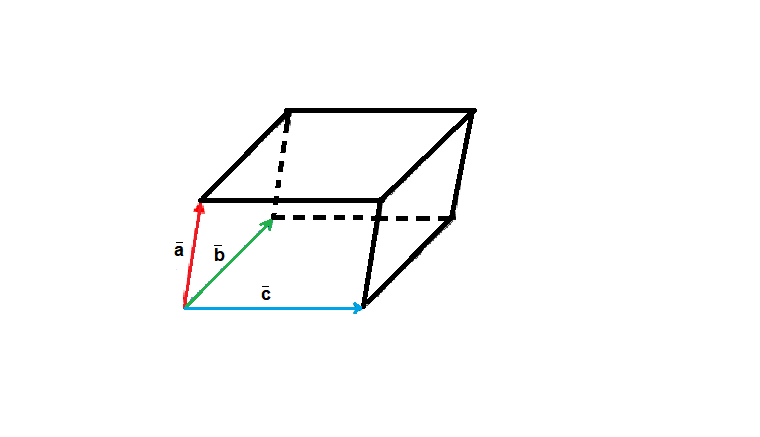
\includegraphics[width=0.55\textwidth]{Parall.png}}
	\caption[Parallelepiped built on three vectors]{Parallelepiped built on three vectors.}
	\label{fig:Pararll}
\end{figure}

Since each column and row represents the coordinates of a unit vector, the length of the vectors defined by the rows and columns of the rotation matrix is 1. The determinant of the rotation matrix is +1 for a right-handed frame of reference and -1 for a left-handed one. Thus, if the determinant value is -1, the image will be inverted for a right-handed frame of reference.\\

\section{Transformation Chain}

Let's define the coordinates of the point in the camera coordinat system and in the world coordinat system(the values do not match). Let $M=(x_w,y_w,z_w)$ - point in the world coordinates and $M=(x_c,y_c,z_c)$ - point in the camera coordinates and $t= (O_c, O_w)$ is translation vector between origins. The extrinsic parameters of camera are contained in the rotation matrix R and the translation vector t, they describe the camera position. Figure~\ref{fig:WtoC} is presented for better understanding.


\begin{figure}[h!]
	\centerline{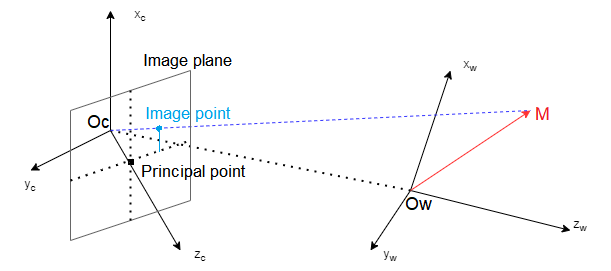
\includegraphics[width=0.55\textwidth]{WtoC.png}}
	\caption[WtoC]{W to C.}
	\label{fig:WtoC}
\end{figure}


We can represent points using this equality:
\begin{equation*}
\left(
\begin{array}{ccc}
	x_c\\
	y_c\\
	z_c
\end{array}
\right) =
t +
R\left(
\begin{array}{ccc}
	x_w\\
	y_w\\
	z_w
\end{array}
\right)
\end{equation*}

We can transform equation in the form below using homogeneous coordinates~\cite{Stricker2021}.:

\begin{equation*}
	\left(
	\begin{array}{ccc}
		x_c\\
		y_c\\
		z_c\\
		1
	\end{array}
	\right) =
	\left(
	\begin{array}{ccc}
		R & t\\
		0_{3}^T & 1
	\end{array}
	\right)
	\left(
	\begin{array}{ccc}
		x_w\\
		y_w\\
		z_w\\
		1
	\end{array}
	\right) 
\end{equation*}
Now we can get a point in the 3D camera coordinate system, project the point onto the image plane and calculate its position on the image. (Figure~\ref{fig:WtoC})\\
We represent image point $(x_i,y_i)$:\\
$x_i=f{{x_c}\over{z_c}}$\\
$y_i=f{{y_c}\over{z_c}}$\\
We can present this equations in matrix form:
\begin{equation*}
\left(
\begin{array}{ccc}
	x'\\
	y'\\
	z'
\end{array}
\right) =
\left(
\begin{array}{ccc}
	f & 0 & 0\\
	0 & f & 0\\
	0 & 0& 1
\end{array}
\right) 
\left(
\begin{array}{ccc}
	x_c\\
	y_c\\
	z_c
\end{array}
\right) 
\end{equation*}
In this case, perspective projection becomes linear in homogeneous coordinates:
\begin{equation*}
	\left(
	\begin{array}{ccc}
		u\\
		v\\
		w
	\end{array}
	\right) =
	\left(
	\begin{array}{cccc}
		f & 0 & 0 & 0\\
		0 & f & 0 & 0\\
		0 & 0 & 1 & 0
	\end{array}
	\right) 
	\left(
	\begin{array}{ccc}
		x_c\\
		y_c\\
		z_c\\
		1
	\end{array}
	\right) 
\end{equation*}

Obviously, the optical center (principal point)  $(x_0, y_0)$ of the camera may not matched with the center of the image coordinate system, and there may also be a skew. We use principal point $(x_0, y_0)$, s - skew parameter and $\alpha_x = fk_x$, $\alpha_y = fk_y$ - scaling factors, so we can get the calibration matrix K, its contains the intrinsic camera parameters:
\begin{equation*}
	K=
	\left(
	\begin{array}{ccc}
		\alpha_x & s & x_0 \\
		0 & \alpha_y & y_0 \\
		0 & 0 & 1 
	\end{array}
	\right)  
\end{equation*}\\
 We can represent formula:
\begin{equation*}
	\left(
	\begin{array}{ccc}
		u'\\
		v'\\
		w'
	\end{array}
	\right) =
	\left(
	\begin{array}{cccc}
		\alpha_x & s & x_0 & 0\\
		0 & \alpha_y & y_0 & 0\\
		0 & 0 & 1 & 0
	\end{array}
	\right) 
	\left(
	\begin{array}{ccc}
		x_c\\
		y_c\\
		z_c\\
		1
	\end{array}
	\right) = K(I_3|0_3)	\left(
	\begin{array}{ccc}
		x_c\\
		y_c\\
		z_c\\
		1
	\end{array}
	\right) 
\end{equation*}

So we can find the pixel coordinates (u, v):
$x_{pix}={{u'}\over{w'}}; \ y_{pix}={{v'}\over{w'}}$

\section{Implementation}

In your report, show the first image with the following information:\\
- projected points without correction of the distortion in red

\begin{figure}[h!]
	\centerline{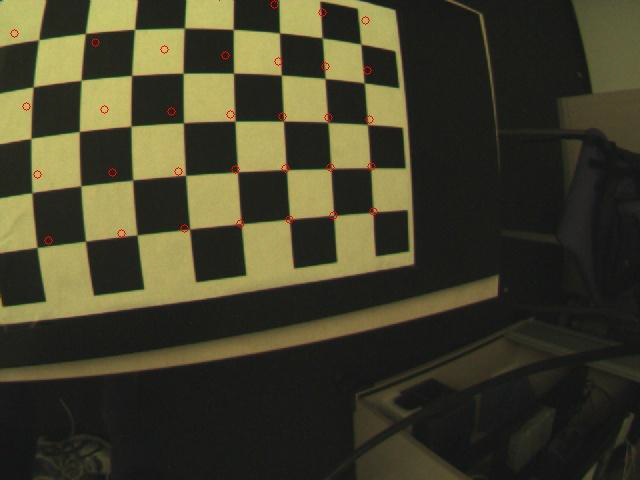
\includegraphics[width=0.55\textwidth]{wCorr.png}}
	\caption[wCorr]{Projected points without correction of the distortion}
	\label{fig:wCorr}
\end{figure}
- projected points with correction of the radial distortion (k1, k2 and k5) in green

\begin{figure}[h!]
	\centerline{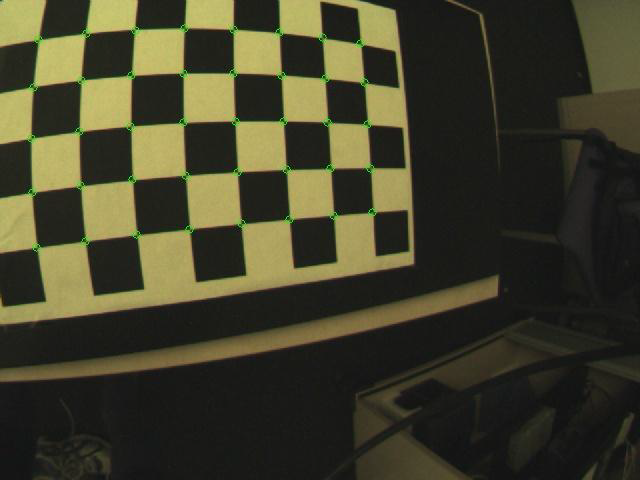
\includegraphics[width=0.55\textwidth]{Corr.png}}
	\caption[Corr]{ Projected points with correction of the radial distortion (k1, k2 and k5)}
	\label{fig:Corr}
\end{figure}

\section{Basic}

In technical reports as well as in scientific manuscripts it is common to work with equations, figures and citations.
Concerning equations, there are several commands available to format them and produce the desired results.
This template focuses on the basics necessary for the exercise reports.
For instance, Eq.~\ref{eq:projection} shows the standard projection of a 3D point $X \in \mathbb{R}^3$ onto a perspective image as
\begin{equation}
 \begin{aligned}
  \lambda x &= P X \\
          x &\sim K \left[ R | t \right] X,
 \end{aligned}
 \label{eq:projection}
\end{equation}
where $P_{3 \times 4}$ is the projection matrix.
Note the alignement on $=$ and $\sim$; this is very useful to neatly display equations.
Still referring to Eq.~\ref{eq:projection}, $K$ is usually called camera matrix and is given by
\begin{equation*}
 K = \left[
 \begin{array}{ccc}
  f_x & s & c_x \\
  0 & f_y & c_y \\
  0 & 0 & 1
 \end{array}
 \right].
 \label{eq:kmatrix}
\end{equation*}

The matrix $K$ holds the \emph{intrinsic} camera parameters whereas the rotation matrix $R_{3 \times 3}$ and the translation vector $t_{3 \times 1}$ hold the \emph{extrinsic} parameters, that is, 
they describe the camera pose as shown in Figure~\ref{fig:stdProj}.
\begin{figure}[ht]
 \centerline{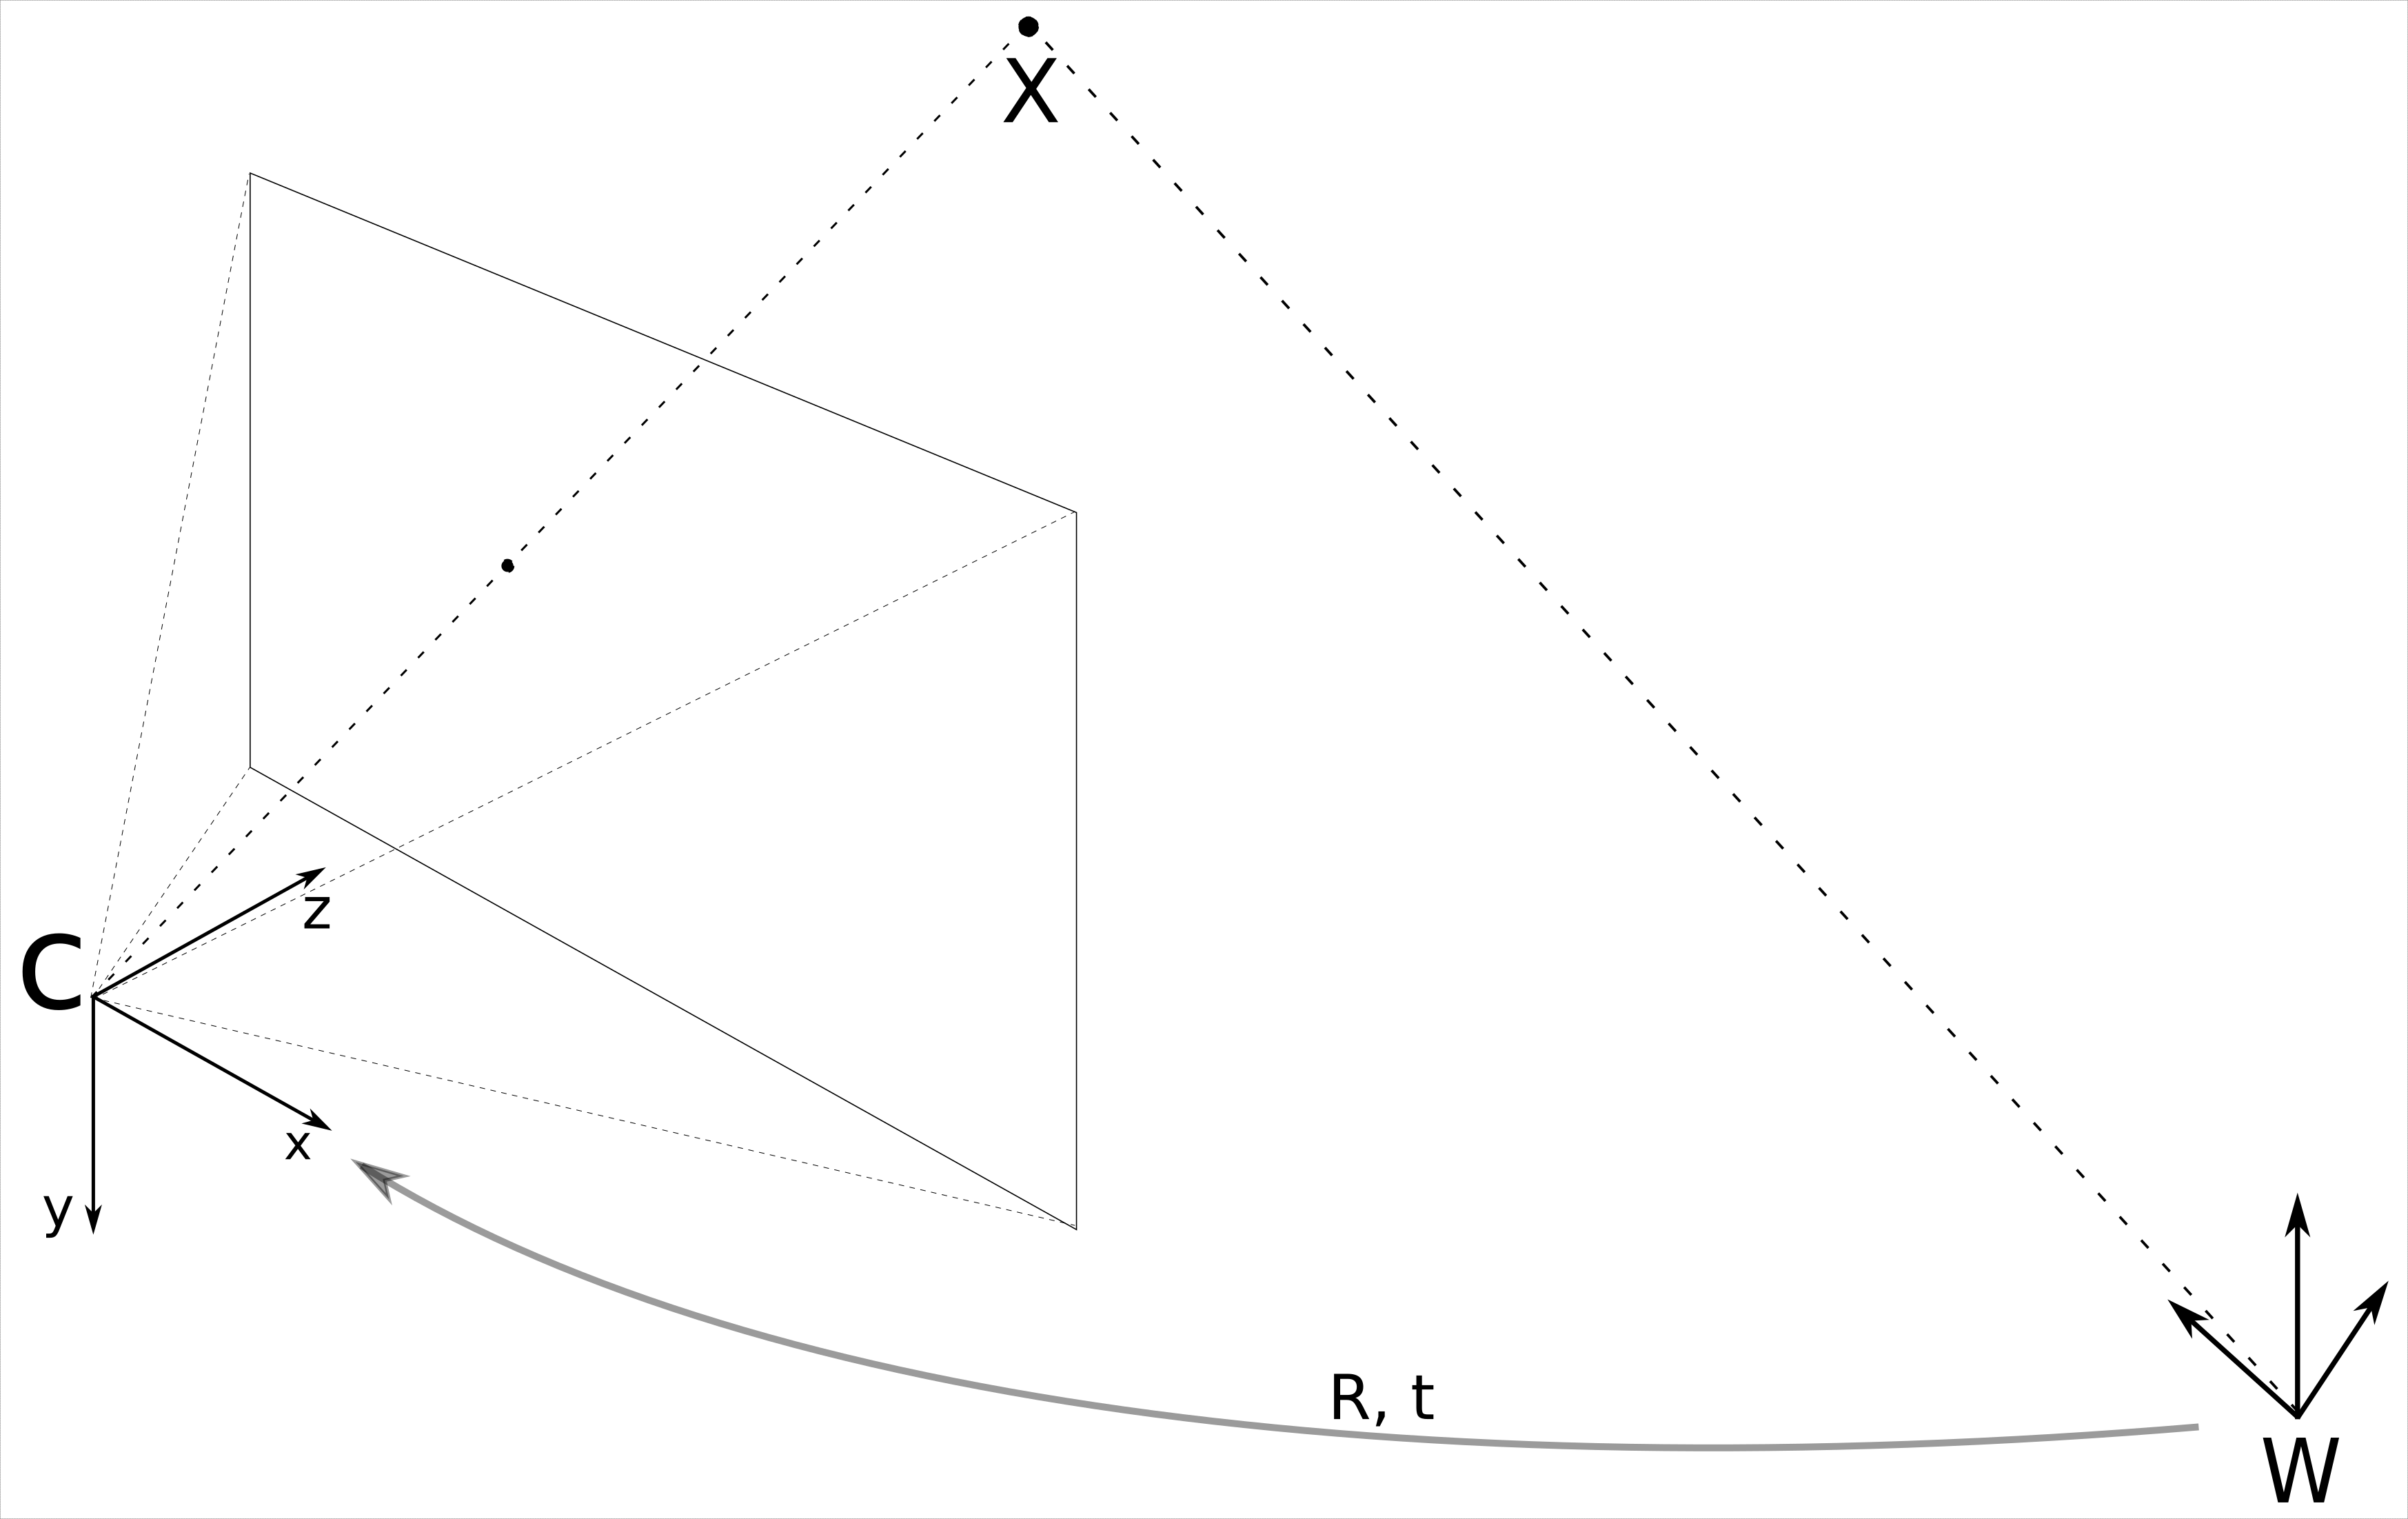
\includegraphics[width=0.65\textwidth]{stdProjection.png}}
 \caption[Standard perspective projection]{Standard perspective projection.}
 \label{fig:stdProj}
\end{figure}

\LaTeX\ also offers convenient ways to arrange multiple pictures into a single figure.
Figure~\ref{fig:inversion} shows an example where an image and the result of processing it are displayed side by side.
\begin{figure}[ht]
 \centerline
 {
  \subfloat[]{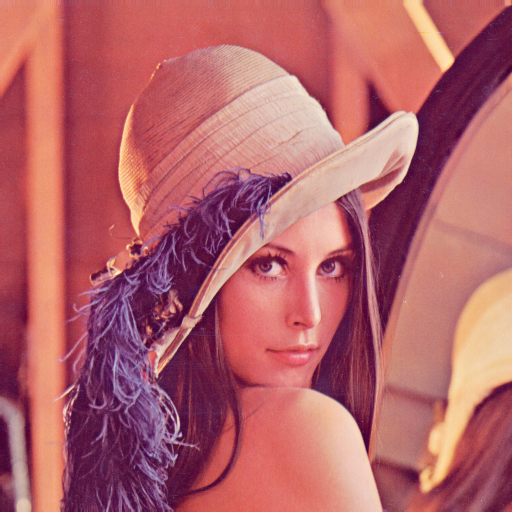
\includegraphics[width=0.35\textwidth]{lena.png}}
  \qquad
  \subfloat[]{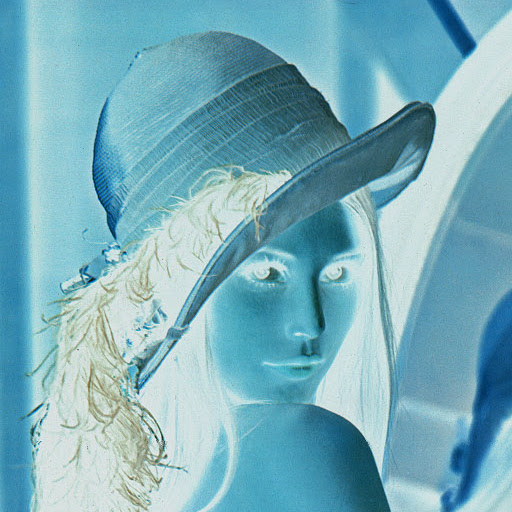
\includegraphics[width=0.35\textwidth]{lenaInverted.png}}
 }
 \caption[Color inversion]{(a) Original image. (b) Result of inverting the colors of (a).}
 \label{fig:inversion}
\end{figure}

Citations are also straightforward.
For example, one of the text books adopted in this lecture can be found in~\cite{Stricker2021}. 

\section{Software}

\subsection{PDF Viewer}
In principle, any pdf viewer will do.
For those who prefer to work with DVI files before creating the final pdf version, Okular (\url{https://okular.kde.org/}) may be a good choice.
DVI files~\footnote{DVI files are specially interesting when working with large documents since the generation of the pdf version may take some time.} are generated quickly and may be seen as an 
intermediate stage between the source file (.tex) and the pdf.

\subsection{Editors}
There are many flavors.
Here are some:
\begin{itemize}
 \item Texmaker (Linux, Windows, Mac);
 \item TeXstudio (Linux, Windows, Mac);
 \item MiKTeX (Windows);
 \item \textbf{Kile} (KDE Linux)
\end{itemize}

\subsection{Image format}
It is recommended to work with either \texttt{png} or \texttt{eps} format.
If you choose the former, beware the generation of DVI files will most likely fail.
In this case, you will need to invoke PDFLatex, which converts the source file directly to pdf.
If you prefer \texttt{eps}, creating DVI files should work smoothly.

\bibliographystyle{plain}
\bibliography{bibliography.bib}
\end{document}